\chapter{Opportunity, Pressure, and the Mirror}

In this School of Hard Knocks interview, curated by LazyingArt LLC, the spectacle comes first and the method comes second. Tom Brady is introduced through rings, awards, and wealth, but the lecture itself steadily pushes away from public magnitude toward a smaller set of hidden mechanisms: use the opportunities actually given, let obscurity build resilience before recognition, rehearse pressure before it arrives, and measure the whole enterprise by the person one becomes. The mathematics here is necessarily light and editorial, because the interview is not blackboard-native. Even so, the transcript invites a precise structure, and it is worth writing that structure down while the sequence is still visible.

\section{Scale First, Then the Reduction}

The host opens in the usual register of scale: the greatest football player of all time, seven Super Bowls, three MVPs, and hundreds of millions of dollars. That opening matters because the lecture's authority depends on the magnitude being real before the explanation turns modest. What follows is not a theory of celebrity. It is Brady's first reduction of visible success back to process.

Asked how he made his millions, he does not begin with endorsements, equity, or post-career businesses. He begins with football itself: hard work on the field, taking hits, getting the ball out quickly, and throwing to teammates. The order is important. The money sits downstream of the machine, not upstream of it.

The next reduction is even more decisive. Brady says, in effect, that he did the best he could with the opportunities he got and refused to compare himself to anybody else. This is the lecture's first real principle, and it can be written with a useful distinction:
\begin{equation}
O_{\text{given}} \neq O_{\text{others}}.
\end{equation}
Here \(O_{\text{given}}\) denotes the opportunities actually available to the agent, while \(O_{\text{others}}\) denotes the opportunities visibly granted elsewhere. The interview's claim is that one does not build a career by emotionally optimizing over the second set.

A cautious editorial compression is therefore
\begin{equation}
\max \operatorname{Use}(O_{\text{given}})
\quad \text{rather than} \quad
\max \operatorname{Complaint}(O_{\text{others}}).
\end{equation}
The point is not to mathematize a moral slogan for its own sake. The point is that Brady's earliest answer already contains a decision rule.

\subsection{Question \& Answer}

\paragraph{Question.} What exactly should we optimize when the world appears to be giving other people more?

\paragraph{Answer.} The lecture's first answer is not comparison but conversion. We should optimize what we do with the opportunities that are actually ours. The host is still speaking in the language of greatness, but Brady has already shifted the chapter into a narrower grammar: attention belongs on the available rep, not the visible unfairness.

\section{Nine Years Before the Pros}

The lecture then moves backward in time. Brady does not present greatness as something that first appeared on Sundays. He says that through high school and college he had to work very hard just to become a starter and then, even later, a contributor. The crucial phrase is that these years taught him resiliency before anyone was paying attention.

The transcript compresses that entire formation period into a rough horizon:
\begin{equation}
T_{\text{apprenticeship}} \approx 9 \ \text{years}.
\end{equation}
This is not a demographic fact about every athlete. It is Brady's own way of naming the long pre-professional interval in which the character of later performance was built.

\paragraph{Claim.} Self-confidence at the professional level was not the starting point.

\paragraph{Mechanism.} Repeated obscurity, effort, and adaptation in earlier years generated the internal structure that later appeared as confidence when the stage became larger.

A light update rule captures the spirit of the claim:
\begin{equation}
B_{t+1} = B_t + \Delta B_t,
\qquad
\Delta B_t > 0 \ \text{after adversity is survived}.
\end{equation}
Here \(B_t\) is not a psychological measurement. It is only an editorial state variable for self-belief. The lecture's point is that belief was accumulated, not granted.

The draft line sharpens the same structure. Asked whether anybody doubted him, Brady answers with institutional arithmetic:
\begin{equation}
N_{\text{teams}} = 32,
\qquad
R_{\text{passed}} = 6.
\end{equation}
The wording is deliberately public. The league's visible judgment arrives before his own long result does. This is why the interview is so careful to say that much of the work happened when no one was paying attention. Public selection and actual potential are not the same object.

\subsection{Question \& Answer}

\paragraph{Question.} How is self-belief formed before success is publicly visible?

\paragraph{Answer.} In this lecture, it is formed the hard way. One works through a long interval in which recognition is thin, feedback is mixed, and status is low. If one survives that interval by finding strategies that actually work, then confidence later appears not as fantasy, but as memory of what has already been overcome.

\section{Failure, Comfort, and Longevity}

Once the lecture has located confidence inside a long apprenticeship, it can say something more exact about failure. Brady does not treat failure as an exception to his success. He treats it as a training medium. Trial and error, repeated mistakes, and the willingness to absorb them become part of the mechanism by which later steadiness is built.

The lightest faithful compression is
\begin{equation}
\text{failure} \to \text{adaptation} \to \text{confidence}.
\end{equation}
Again, this is editorial notation rather than quoted mathematics. But it clarifies the logic of the interview. Confidence is not an inward speech detached from experience. It is the residue left behind by repeated correction.

The same section widens the point through the language of comfort. Brady says that one can wake up every day and live inside comfort and convenience, repeating the same routines. But growth requires moving outside that regime. We may therefore distinguish a comfort domain \(\mathcal C\) from a growth domain \(\mathcal G\):
\begin{equation}
\mathcal C \to \mathcal G.
\end{equation}
The lecture never formalizes a boundary between the two, and we should not pretend that it does. But the direction matters. Success is being tied not to the protection of familiar states, but to repeated departures from them.

The next pivot is from emergence to persistence. Once the lecture has explained how greatness begins, it asks how it lasts. Brady's answer is mentorship and discipline. He names Alex Guerrero in particular and ties longevity to learned bodily care, routine, and sustained attention to health. The lecture's structure is clear: greatness is built once by resilience and then maintained again by discipline. Talent alone does not cover both problems.

\section{Greg Harden and the Arithmetic of Opportunity}

The Greg Harden story is the lecture's cleanest local correction. Brady describes himself as a sophomore in college, frustrated, complaining, and preoccupied with the chances being given to other people. Harden interrupts that posture bluntly and redirects him to the opportunities actually in hand. The memorable example is not grand. It is small. If the practice gives you three real chances, then use those three chances.

That logic can be written without violence:
\begin{equation}
\operatorname{Focus}_t = O_{\text{given},t},
\qquad
\operatorname{Action}_t = \operatorname{Use}(O_{\text{given},t}).
\end{equation}
The precision matters because the story is not merely motivational. It changes the variable being optimized. Complaint had been indexed to what others received. Harden moves Brady to the local set of reps and asks him to maximize there.

\paragraph{Anecdote.} Brady complains that others are receiving more opportunity.

\paragraph{Claim.} The path forward is not to win the comparison argument, but to use the chances that are actually present.

\paragraph{Mechanism.} Attention and effort are reallocated from envy to available action.

This is the natural place for accountability to enter. The interview says it very directly: nobody is coming to save you. The stronger version is not isolated individualism, but responsibility to oneself and to the people who matter. Still, the internal spine is unmistakable. One cannot outsource the use of one's own opportunities.

\subsection{Question \& Answer}

\paragraph{Question.} What do we do when the distribution of opportunity feels unfair?

\paragraph{Answer.} The lecture's answer is not to deny the asymmetry. It is to refuse to let the asymmetry determine our entire behavior. We do not need to pretend the world is evenly allocated. We need to stop letting visible inequality paralyze the use of the reps we actually possess.

At this point the video itself is interrupted by a long host-run promotion. That interruption belongs to the economics of the platform rather than to Brady's argument. We therefore mark it and move on. When the interview returns, the question has changed. The lecture now wants to know not how we respond to unfairness, but how we train for pressure.

\section{Pressure Before Pressure}

This is the mathematically strongest stretch in the lecture. Brady's answer is not that one becomes brave only when the large moment arrives. One becomes usable under pressure by repeatedly placing oneself in pressure-like states before the official pressure exists.

He says that he treated practice like a game. If they scored a touchdown in practice, he celebrated as though it were game day. He wanted the emotions of game day to become familiar even when it was not game day. That is already a state-matching claim:
\begin{equation}
S_{\text{practice}} \sim S_{\text{game}},
\end{equation}
where \(\sim\) means deliberate approximation of stakes and emotional load, not literal equality.

The lecture then becomes even more concrete. In the offseason, throwing with teammates, he would assign the rep an exact dramatic form: fourth down, fourth and seven, one shot to win the Super Bowl. Let us write the local state as
\begin{equation}
d = 4,
\qquad
y = 7,
\qquad
\text{task} = \text{score now or lose}.
\end{equation}
This is not football notation for its own sake. It is a method for importing consequence into a rep that would otherwise remain ordinary.

The underlying causal chain is the real object:
\begin{equation}
\text{simulated stakes}
\to
\text{emotional familiarity}
\to
\text{embodied readiness}.
\end{equation}
The lecture's language is that by the time the real moment arrives in February, the body already knows and has already been programmed for that experience. We should keep that phrasing metaphor-sensitive. It is not a neuroscience theorem. It is an experiential claim: the high-pressure state is less alien because it has been rehearsed.

\begin{figure}[h]
\centering
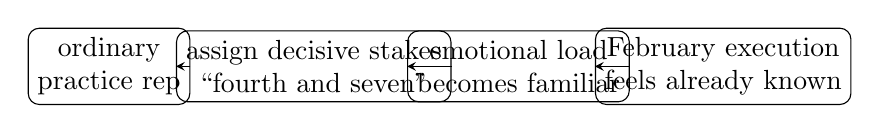
\begin{tikzpicture}[node distance=2.6cm, >=stealth]
\node[draw, rounded corners, align=center] (a) {ordinary\\practice rep};
\node[draw, rounded corners, right of=a, align=center] (b) {assign decisive stakes\\``fourth and seven''};
\node[draw, rounded corners, right of=b, align=center] (c) {emotional load\\becomes familiar};
\node[draw, rounded corners, right of=c, align=center] (d) {February execution\\feels already known};

\draw[->] (a) -- (b);
\draw[->] (b) -- (c);
\draw[->] (c) -- (d);
\end{tikzpicture}
\caption{Transcript-derived schematic of Brady's pressure-training loop. The lecture's claim is not that practice and game are identical, but that pressure becomes trainable when ordinary reps are repeatedly loaded with decisive stakes.}
\end{figure}

\subsection{Question \& Answer}

\paragraph{Question.} How do we prepare for pressure before the real pressure arrives?

\paragraph{Answer.} We do not wait passively for the large moment and hope courage appears on demand. We construct smaller moments in advance and make them carry enough consequence that our emotions, decisions, and bodily habits begin to treat them as real. Then when the official moment arrives, it is still serious, but it is not wholly new.

\section{Super Bowl 51 and the Refusal to Quit}

The pressure doctrine now receives its extreme test case. The host asks Brady to go back to Super Bowl 51, invoking the famous \(28\text{-}3\) deficit. Brady's answer, however, first names a different state: \(21\text{-}3\). That sequence matters and should be kept rather than flattened.

Let
\begin{equation}
D = \text{opponent score} - \text{own score}.
\end{equation}
Then the lecture's two marked states become
\begin{align}
D_{21\text{-}3} &= 21-3 = 18,\\
D_{28\text{-}3} &= 28-3 = 25.
\end{align}
This is our explicit worked example. The pressure problem does not merely persist; it worsens. Belichick's line that 21 points would not be enough functions as a refusal to let the present deficit dictate the future. Brady then concedes the next thought honestly: once it becomes \(28\text{-}3\), perhaps 28 is enough after all.

That honesty matters because it prevents the lecture from becoming mythological. He is not saying that doubt vanished. He is saying that quitting remained prohibited even after the state worsened. The logic is plain:
\begin{equation}
D \uparrow
\not\Rightarrow
\text{quit}.
\end{equation}
Instead the lecture insists on a harder update rule:
\begin{equation}
D \uparrow
\quad \text{while} \quad
\text{fight} = \text{constant}.
\end{equation}
This is only symbolic, but it names the essential feature of the answer. Resilience is not tested when the numbers improve. It is tested when they deteriorate and action must continue anyway.

The section then broadens from one game to competition itself. Brady says that anyone can play one game, but sustained excellence across a season requires an entirely different level of discipline. The transcript gives a hierarchy of season outcomes:
\begin{equation}
E_{4\text{-}13} < E_{9\text{-}8} < E_{12\text{-}5} < E_{15\text{-}2}.
\end{equation}
We should treat this as qualitative rather than statistical. Still, the ranking matters. The effort needed to survive a season at elite level is not marginally greater than the effort needed to drift through it. It is categorically greater. That is why Brady immediately moves to habits, actions, and choices:
\begin{equation}
\text{habits} \to \text{actions} \to \text{choices} \to \text{season outcome}.
\end{equation}
This is the lecture's second major scale correction. Public records look like outputs. Brady treats them as cumulative consequences of daily structure.

\section{The Father, the Mirror, and the End of Comparison}

The interview could have ended with competition alone, but it does not. It returns to a different register: heroism, fatherhood, transmission, and the self one can tolerate seeing in the mirror.

Brady names his father as his hero and explains the influence in practical terms: steadiness, presence, belief, and the provision of opportunity. The point is not abstract gratitude. It is inheritance of standard. What he wishes to pass on to his children is not merely achievement, but belief in them and the durable presence that made his own development possible.

That movement prepares the final rule of the lecture. If he had one guiding principle left for the younger generation, it would be to be proud of the person in the mirror every day. This gives the chapter its last objective function:
\begin{equation}
J_{\text{self}}
=
\text{be able to respect the person in the mirror}.
\end{equation}
The lecture then sharpens it still further. The life one leads is the lesson one teaches. Others watch not only what one says, but what one repeatedly does. Integrity, resilience, care, and joy are therefore not decorative virtues after achievement. They are the final form that achievement must take if it is to become worth transmitting.

It is important that the lecture ends here rather than at \(28\text{-}3\). The comeback is magnificent, but it is not the final standard. The final standard is what kind of person the long struggle, the hidden work, the repeated pressure, and the public success have produced.

\section{Summary}

The lecture begins with legend and ends with judgment. In between, it gives a coherent sequence. First, do not compare yourself into paralysis; use the opportunities you actually receive. Second, let obscurity and adversity build resilience before the public notices you. Third, do not think of pressure as a rare monster that appears only on the biggest day. Train it in advance by assigning ordinary reps extraordinary consequence. Fourth, when the state worsens, do not confuse worsening conditions with permission to quit. And finally, do not mistake public praise for the true objective. The final criterion is not whether the world calls one great, but whether one can meet the person in the mirror without evasion.